\documentclass[a4paper]{article}
\usepackage[utf8x]{inputenc}
\usepackage[T1,T2A]{fontenc}
\usepackage[russian]{babel}
\usepackage{hyperref}
\usepackage{indentfirst}
\usepackage{listings}
\usepackage{color}
\usepackage{here}
\usepackage{array}
\usepackage{multirow}
\usepackage{graphicx}
\usepackage[space]{grffile}

\usepackage{caption}
\renewcommand{\lstlistingname}{Программа} % заголовок листингов кода

\usepackage{listings}
\lstset{ %
extendedchars=\true,
keepspaces=true,
language=bash,					% choose the language of the code
basicstyle=\footnotesize,		% the size of the fonts that are used for the code
numbers=left,					% where to put the line-numbers
numberstyle=\footnotesize,		% the size of the fonts that are used for the line-numbers
stepnumber=1,					% the step between two line-numbers. If it is 1 each line will be numbered
numbersep=5pt,					% how far the line-numbers are from the code
backgroundcolor=\color{white},	% choose the background color. You must add \usepackage{color}
showspaces=false				% show spaces adding particular underscores
showstringspaces=false,			% underline spaces within strings
showtabs=false,					% show tabs within strings adding particular underscores
frame=single,           		% adds a frame around the code
tabsize=2,						% sets default tabsize to 2 spaces
captionpos=b,					% sets the caption-position to bottom
breaklines=true,				% sets automatic line breaking
breakatwhitespace=false,		% sets if automatic breaks should only happen at whitespace
escapeinside={\%*}{*)},			% if you want to add a comment within your code
postbreak=\raisebox{0ex}[0ex][0ex]{\ensuremath{\color{red}\hookrightarrow\space}}
}

\usepackage[left=2cm,right=2cm,
top=2cm,bottom=2cm,bindingoffset=0cm]{geometry}



\begin{document}	% начало документа

\begin{titlepage}	% начало титульной страницы

	\begin{center}		% выравнивание по центру

		\large Санкт-Петербургский Политехнический Университет Петра Великого\\
		\large Институт компьютерных наук и технологий \\
		\large Кафедра компьютерных систем и программных технологий\\[6cm]
		% название института, затем отступ 6см
		
		\huge Методы и средства защиты информации\\[0.5cm] % название работы, затем отступ 0,5см
		\large Отчет по лабораторной работе №1\\[0.1cm]
		\large Программа для шифрования и подписи GPG, пакет Gpg4win\\[5cm]

	\end{center}


	\begin{flushright} % выравнивание по правому краю
		\begin{minipage}{0.25\textwidth} % врезка в половину ширины текста
			\begin{flushleft} % выровнять её содержимое по левому краю

				\large\textbf{Работу выполнил:}\\
				\large Косолапов С.А.\\
				\large {Группа:} 53501/3\\
				
				\large \textbf{Преподаватель:}\\
				\large Вылегжанина К.Д.

			\end{flushleft}
		\end{minipage}
	\end{flushright}
	
	\vfill % заполнить всё доступное ниже пространство

	\begin{center}
	\large Санкт-Петербург\\
	\large \the\year % вывести дату
	\end{center} % закончить выравнивание по центру

\thispagestyle{empty} % не нумеровать страницу
\end{titlepage} % конец титульной страницы

\vfill % заполнить всё доступное ниже пространство


% Содержание
\tableofcontents
\newpage



\section{Цель работы}

Научиться создавать сертификаты, шифровать файлы и ставить ЭЦП.

\section{Программа работы}

\begin{itemize}

\item Изучить документацию, запустить графическую оболочку Kleopatra

\item Создать ключевую пару OpenPGP (File → New Certificate)

\item Экспортировать сетрификат (File → Export Certificate)

\item Поставить ЭЦП на файл (File → Sign/Encrypt Files)

\item Взять сертификат кого-либо из коллег, зашифровать и подписать для него какой-либо текст, предоставить свой сертификат, убедиться, что ему удалось получить открытый текст, проверить подпись

\item Предыдущий пункт наоборот

\item Используя GNU Privacy handbook (ссылка в материалах) потренироваться в использовании gpg через интерфейс командной строки, без использования графических оболочек.

\end{itemize}


\section{Теоретическая информация}


\section{Ход выполнения работы}

\subsection{GPG и Оболочка Kleopatra}

PGP - сокращение от Pretty Good Privacy, в переводе - ''достаточно хорошая секретность'', название программы , написанной Филиппом Циммерманном в 1991 году. Эта программа позволяла удобным образом использовать шифрование данных. За её написание Циммермана пытались судить в США, программу перекупали друг у друга разные фирмы, в данный момент PGP принадлежит фирме Symantec, и PGP является коммерческой программой.


Kleopatra - менеджер сертификатов для OpenPGP (одной из реализаций PGP) и x.509 с GUI. Есть реализации под многие ОС семейств Windows, Linux.

\begin{figure}[H]
	\begin{center}
		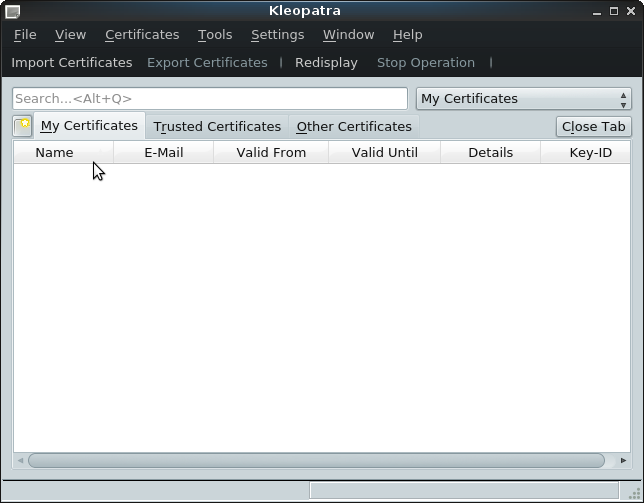
\includegraphics[scale=0.5]{pics/Screenshot at 2016-04-18 00:20:42.png}
		\caption{Внешний вид программы Kleopatra (без сертификатов)} 
		\label{pic:pic_name} % название для ссылок внутри кода
	\end{center}
\end{figure}

Как видим, основную часть окна занимает ListBox с отображаемыми сертификатами. Можем выбрать между "Моими сертификатами", "Доверенными сертификатами" и "Другими сертификатами". Ниже меню расположены кнопки, позволяющие произвести импорт/экспорт сертификата, обновить ("Повторно отобразить") сертификаты и "Остановить операцию".

\subsection{Создание нового сертификата}

Создать новый сертификат можно, нажав клавиши Ctrl+N или через меню File -> New Sertificate. В этом случае появится окно, позволяющее выбрать, что же, собственно, мы хотим создать - GPG или x509 сертификат.

\begin{figure}[H]
	\begin{center}
		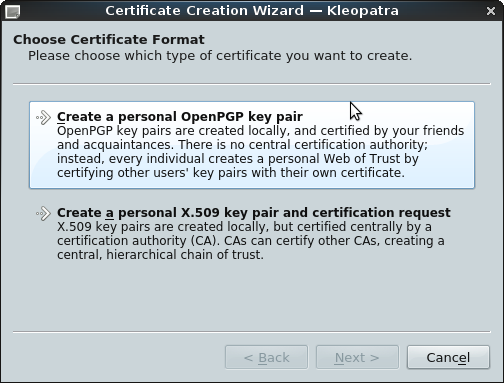
\includegraphics[scale=0.5]{pics/Screenshot at 2016-04-18 00:22:00.png}
		\caption{Окно выбора типа сертификата при создании} 
		\label{pic:pic_name} % название для ссылок внутри кода
	\end{center}
\end{figure}

Выбираем создание пары ключей OpenPGP (первый пункт).

Появляется окно, в котором нужно указать характеристики сертификата - владельца, его адрес электронной почты и, при необходимости, комментарий.

\begin{figure}[H]
	\begin{center}
		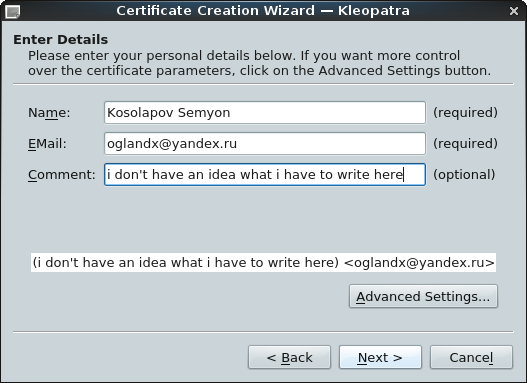
\includegraphics[scale=0.5]{pics/Screenshot at 2016-04-18 00:40:50.png}
		\caption{Окно ввода персональных данных при создании сертификата GPG} 
		\label{pic:pic_name} % название для ссылок внутри кода
	\end{center}
\end{figure}

Также можно выбрать дополнительные настройки. Можно указать тип алгоритма шифрования (RSA/DSA/ECDSA) и его длину. В данном случае выбран стандартный вариант - 2048 бит RSA. Ниже можно указать цель использования сертификата и дату окончания его срока действия.

\begin{figure}[H]
	\begin{center}
		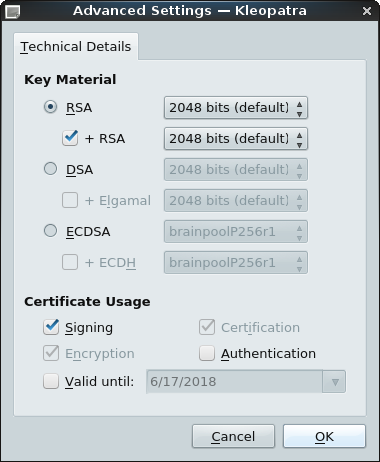
\includegraphics[scale=0.5]{pics/Screenshot at 2016-06-17 13:41:46.png}
		\caption{Окно указания технических деталей GPG} 
		\label{pic:pic_name} % название для ссылок внутри кода
	\end{center}
\end{figure}

Далее визард предоставляет возможность ещё раз просмотреть введённые параметры.

\begin{figure}[H]
	\begin{center}
		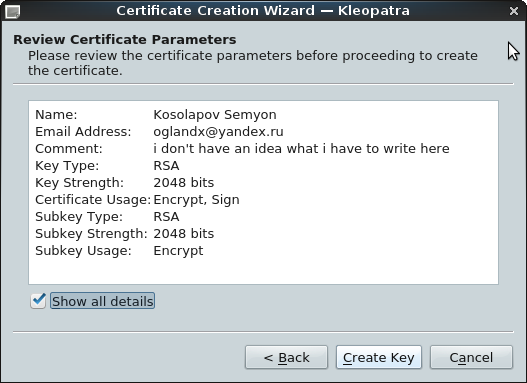
\includegraphics[scale=0.5]{pics/Screenshot at 2016-04-18 00:41:00.png}
		\caption{Ревью параметров сертификата (с просмотром дополнительных параметров)} 
		\label{pic:pic_name} % название для ссылок внутри кода
	\end{center}
\end{figure}

Далее производится создание пары ключей для сертификата. 

\begin{figure}[H]
	\begin{center}
		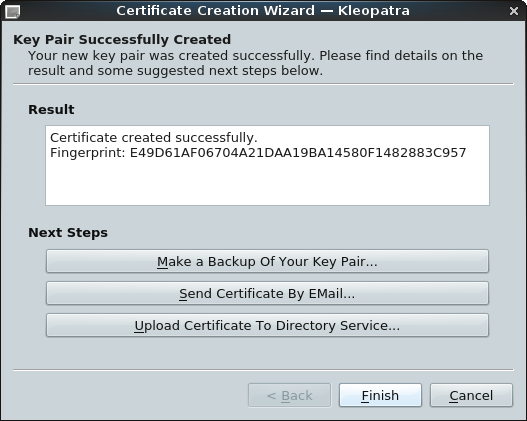
\includegraphics[scale=0.5]{pics/Screenshot at 2016-04-18 00:44:47.png}
		\caption{Окно, демонстрирующее успешное создание ключа} 
		\label{pic:pic_name} % название для ссылок внутри кода
	\end{center}
\end{figure}

Можем просмотреть ключи сертификата.

\begin{figure}[H]
	\begin{center}
		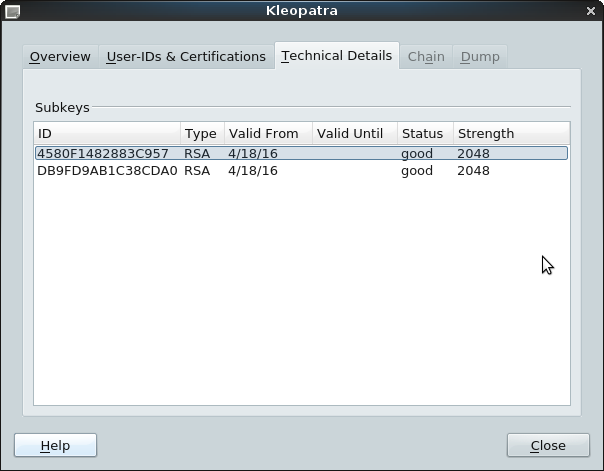
\includegraphics[scale=0.7]{pics/Screenshot at 2016-04-18 00:47:43.png}
		\caption{Просмотр ключей сертификата} 
		\label{pic:pic_name} % название для ссылок внутри кода
	\end{center}
\end{figure}

После создания сертификат стал отображаться в главном окне в списке сертификатов. Там можно просмотреть его характеристики, удалить и т.д.

\begin{figure}[H]
	\begin{center}
		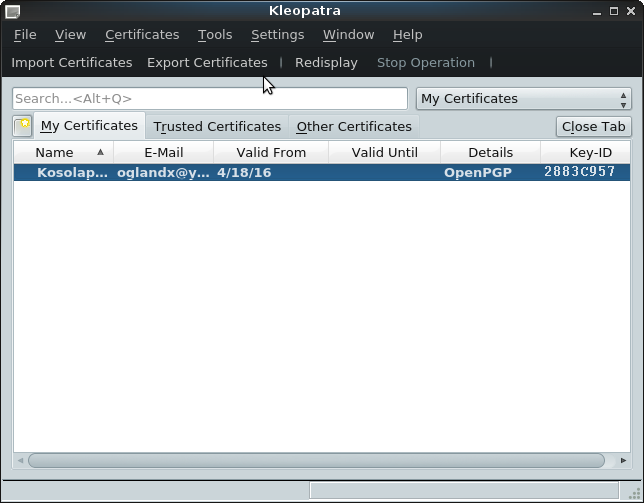
\includegraphics[scale=0.5]{pics/Screenshot at 2016-04-18 00:52:12.png}
		\caption{Вид главного окна после создания сертификата} 
		\label{pic:pic_name} % название для ссылок внутри кода
	\end{center}
\end{figure}


\subsection{Экспорт сертификата}

В после того, как сертификат был создан, можем его экспортировать. Для этого нужно нажать на кнопку "Экспортировать" в верхней части экрана. Появится диалог сохранения.

\begin{figure}[H]
	\begin{center}
		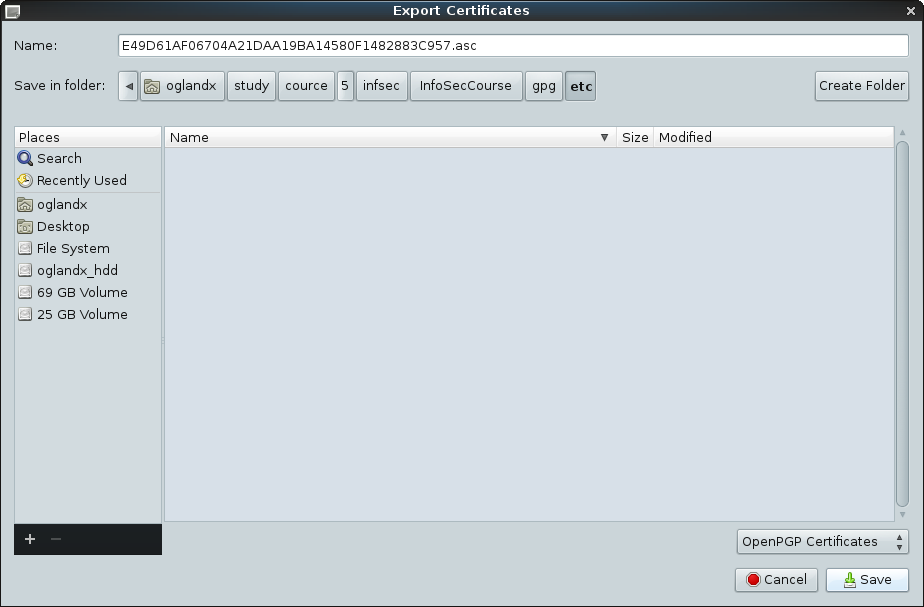
\includegraphics[scale=0.5]{pics/Screenshot at 2016-04-18 00:52:52.png}
		\caption{Выбор директории для сохранения сертификата} 
		\label{pic:pic_name} % название для ссылок внутри кода
	\end{center}
\end{figure}


\subsection{Установка ЭЦП на файл}


Далее можем установить ЭЦП на файл, который, для начала, нужно выбрать.

\begin{figure}[H]
	\begin{center}
		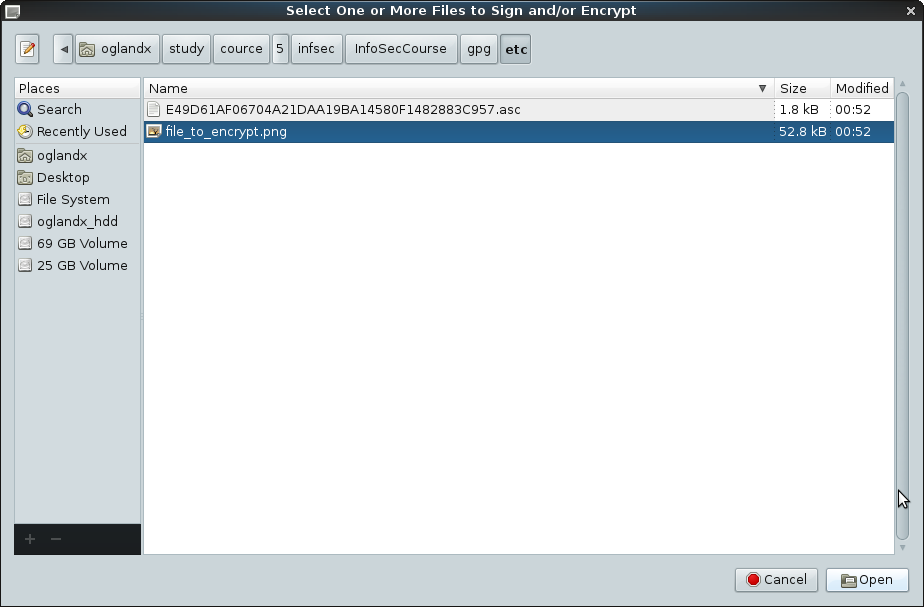
\includegraphics[scale=0.5]{pics/Screenshot at 2016-04-18 00:56:27.png}
		\caption{Выбор файла для установки ЭЦП} 
		\label{pic:pic_name} % название для ссылок внутри кода
	\end{center}
\end{figure}

После чего появится диалог, в котором можно выбрать действия, которые мы хотим произвести. 

\begin{figure}[H]
	\begin{center}
		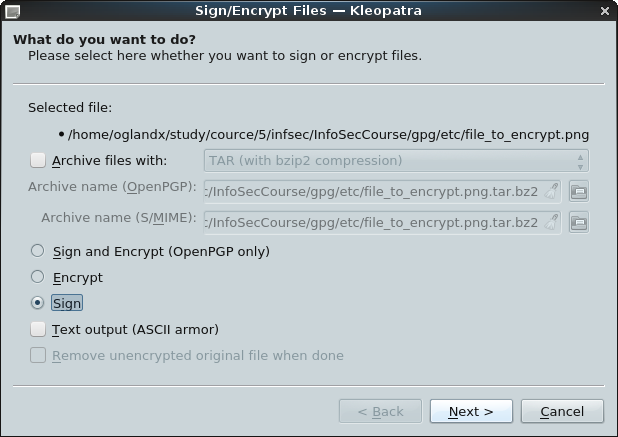
\includegraphics[scale=0.5]{pics/sign.png}
		\caption{Выбор параметров} 
		\label{pic:pic_name} % название для ссылок внутри кода
	\end{center}
\end{figure}

Установим, что хотим подписать, после чего нажмём next.

\begin{figure}[H]
	\begin{center}
		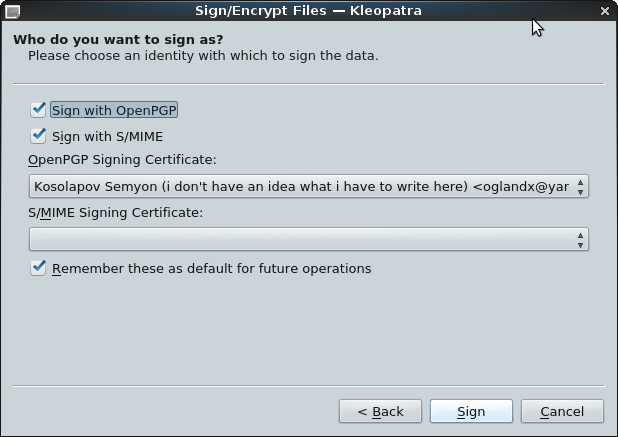
\includegraphics[scale=0.5]{pics/sign_signing.png}
		\caption{Выбор параметров подписи} 
		\label{pic:pic_name} % название для ссылок внутри кода
	\end{center}
\end{figure}

После выбора параметров подписи и ввода passphrase, получаем уведомление об успешности операции:

\begin{figure}[H]
	\begin{center}
		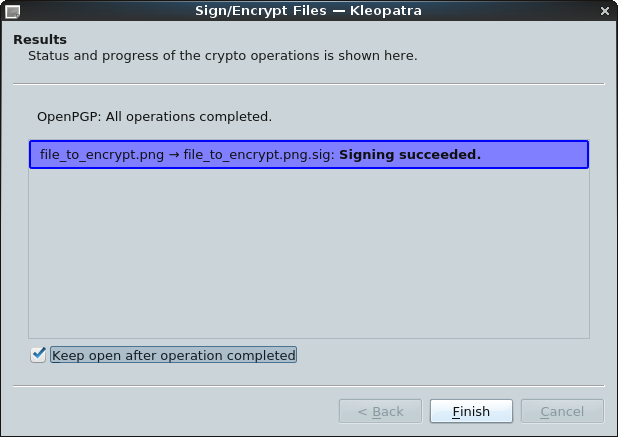
\includegraphics[scale=0.5]{pics/signing_successful.png}
		\caption{Выбор параметров подписи} 
		\label{pic:pic_name} % название для ссылок внутри кода
	\end{center}
\end{figure}

Можем посмотреть, что за файл был создан:

\begin{figure}[H]
	\begin{center}
		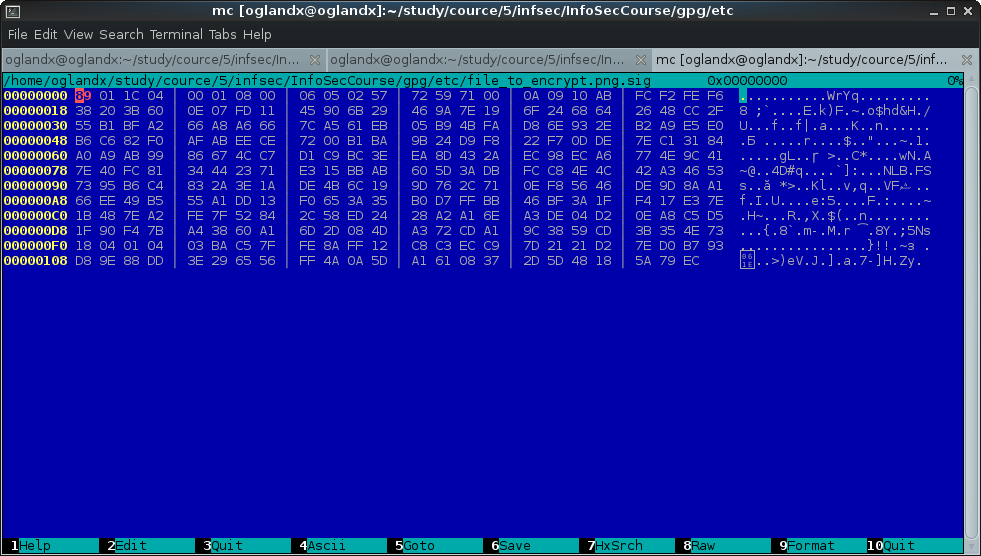
\includegraphics[scale=0.5]{pics/content_of_sig.png}
		\caption{Содержимое sig-файла} 
		\label{pic:pic_name} % название для ссылок внутри кода
	\end{center}
\end{figure}

Как видим, файл имеет довольно небольшой размер. Оригинальный файл должен находиться в одной директории с файлом *.sig.

\subsection{Шифрование файла}

Так же, как и в предыдущем пункте, выбираем файл. После этого в диалоге выбираем encrypt вместо sign.

\begin{figure}[H]
	\begin{center}
		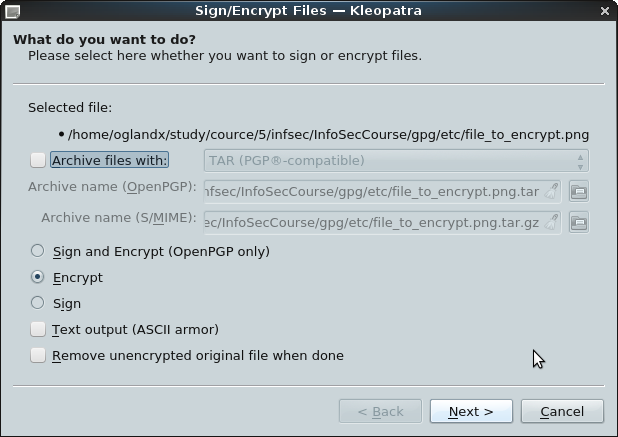
\includegraphics[scale=0.5]{pics/Screenshot at 2016-04-18 00:56:45.png}
		\caption{Выбор опции шифрования} 
		\label{pic:pic_name} % название для ссылок внутри кода
	\end{center}
\end{figure}

Далее предоставляется возможность выбрать сертификат.

\begin{figure}[H]
	\begin{center}
		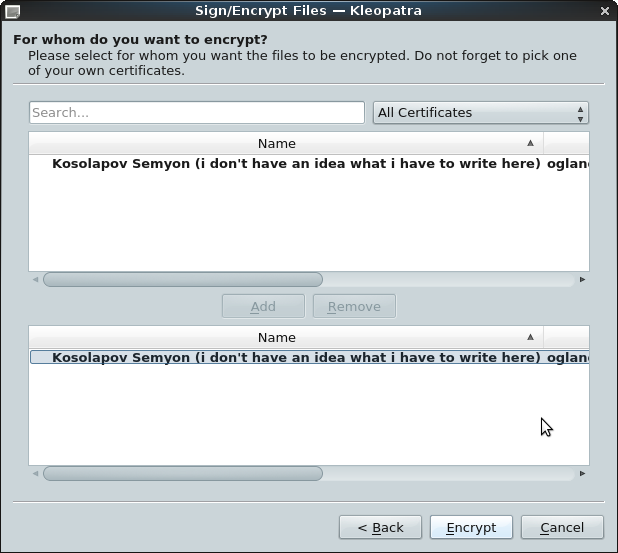
\includegraphics[scale=0.5]{pics/Screenshot at 2016-04-18 00:56:58.png}
		\caption{Выбор сертификата} 
		\label{pic:pic_name} % название для ссылок внутри кода
	\end{center}
\end{figure}

После чего в диалоге появляется сообщение об успешности проведённой операции.

\begin{figure}[H]
	\begin{center}
		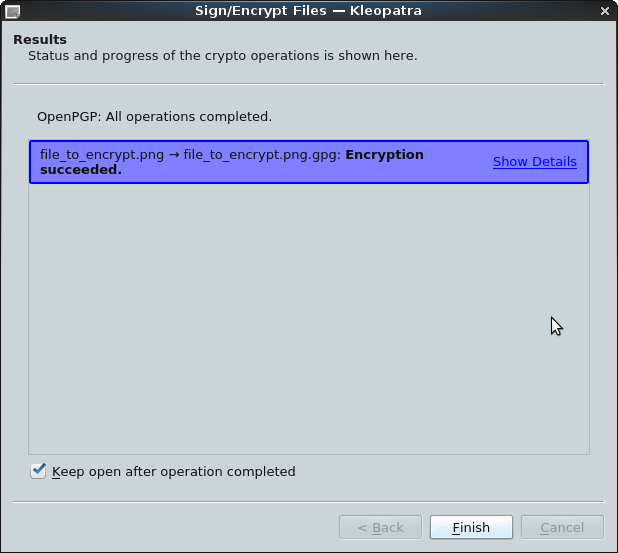
\includegraphics[scale=0.5]{pics/Screenshot at 2016-04-18 00:57:07.png}
		\caption{Шифрование прошло успешно} 
		\label{pic:pic_name} % название для ссылок внутри кода
	\end{center}
\end{figure}

В результате, получили файл с расширением *.gpg.

\begin{figure}[H]
	\begin{center}
		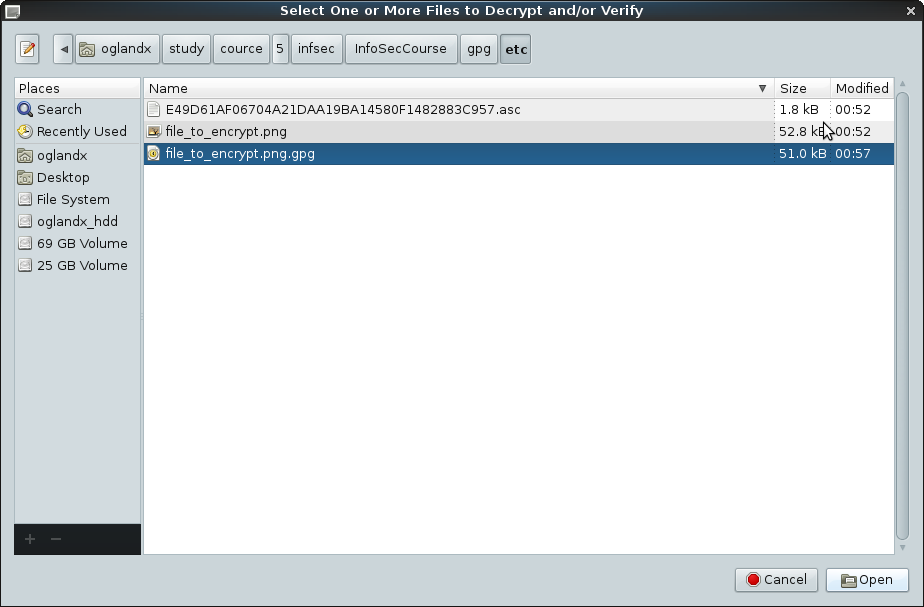
\includegraphics[scale=0.5]{pics/Screenshot at 2016-04-18 01:00:22.png}
		\caption{Файл с расширением .gpg создан после шифрования} 
		\label{pic:pic_name} % название для ссылок внутри кода
	\end{center}
\end{figure}

Далее можем попробовать расшифровать файл. Для этого выбираем Decrypt в диалоге Decrypt/Verify Files. Далее:

\begin{figure}[H]
	\begin{center}
		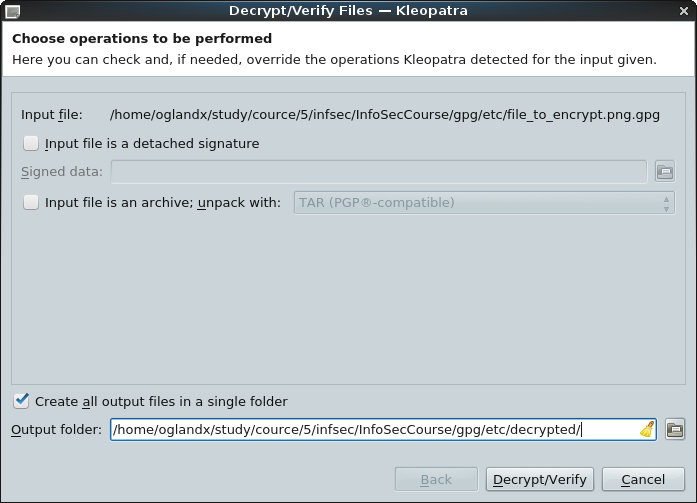
\includegraphics[scale=0.5]{pics/Screenshot at 2016-04-18 01:01:11.png}
		\caption{Дешифрование файла} 
		\label{pic:pic_name} % название для ссылок внутри кода
	\end{center}
\end{figure}

После нажатия на Decrypt/Verify, файл успешно расшифрован.

\subsection{Зашифровать и подписать текст и вместе с сертификатом предоставить коллеге для расшифровки}

Создадим файл с текстом для подписи.

Далее откроем диалог Sign/Encrypt выберем Sign and Encrypt.

\begin{figure}[H]
	\begin{center}
		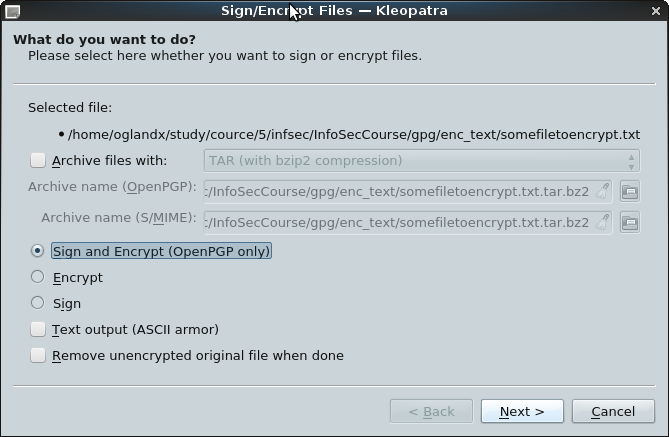
\includegraphics[scale=0.5]{pics/sig_enc.png}
		\caption{Выбор Sgin and Encrypt} 
		\label{pic:pic_name} % название для ссылок внутри кода
	\end{center}
\end{figure}

Выберем сертификат для шифрования.

\begin{figure}[H]
	\begin{center}
		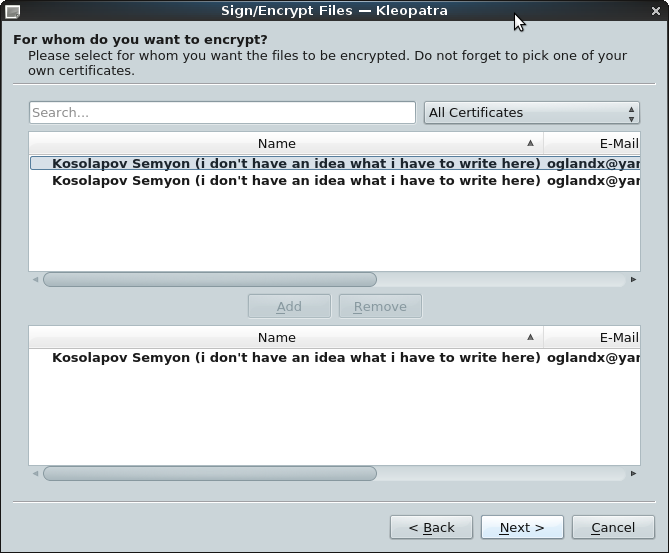
\includegraphics[scale=0.5]{pics/sig_enc_cert.png}
		\caption{Выбор сертификата для шифрования} 
		\label{pic:pic_name} % название для ссылок внутри кода
	\end{center}
\end{figure}

Выберем сертификат для подписи.

\begin{figure}[H]
	\begin{center}
		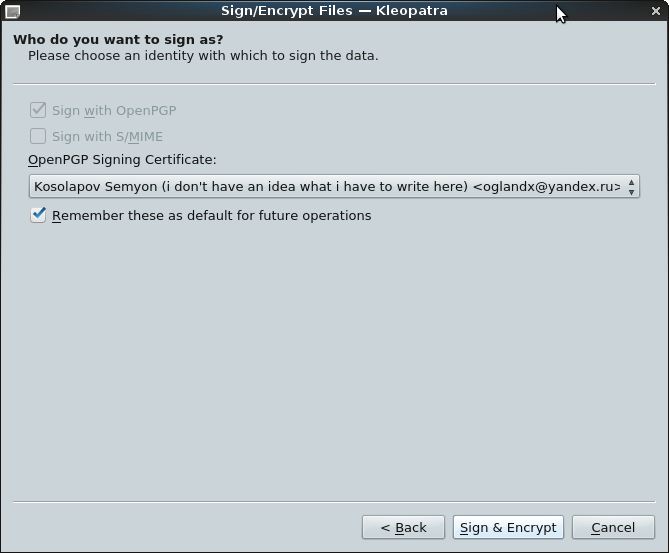
\includegraphics[scale=0.5]{pics/sig_enc_enc.png}
		\caption{Выбор сертификата для подписи} 
		\label{pic:pic_name} % название для ссылок внутри кода
	\end{center}
\end{figure}

В результате - файл успешно подписан и зашифрован.

\begin{figure}[H]
	\begin{center}
		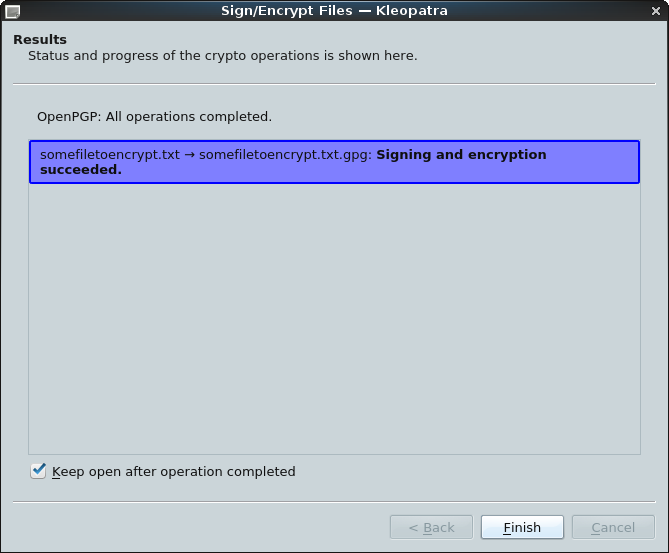
\includegraphics[scale=0.5]{pics/sig_enc_succeeded.png}
		\caption{Операция прошла успешно} 
		\label{pic:pic_name} % название для ссылок внутри кода
	\end{center}
\end{figure}

\subsection{Использование GPG посредством командной строки}

Сначала посмотрим, что умеет gpg, выведя help.

\lstinputlisting[numbers=none, keywords={}, lastline=85]{logs/console.txt}

Затем создадим новый сертификат. Создание проходит в интерактивном режиме.

\lstinputlisting[numbers=none, keywords={}, firstline=87, lastline=121]{logs/console.txt}

Просмотрим имеющиеся подписи и ключи.

\lstinputlisting[numbers=none, keywords={}, firstline=124, lastline=158]{logs/console.txt}

Затем зашифруем и расшифруем файл.

\lstinputlisting[numbers=none, keywords={}, firstline=160, lastline=171]{logs/console.txt}

Как видим, cmp не имеет вывода, значит файлы идентичны.

\section{Выводы}

Электронная подпись важных документов и документов, сохранение целостности которых принципиально, необходима. На данный момент она широко используется и, вместе с тем, средства, позволяющие управлять электронной подписью, имеют простой и удобный интерфейс. Причём это касается как графического интерфейса, так и консольного варианта.

GPG и её реализация OpenGPG является одним из вариантов реализации PGP. Оболочка Kleopatra, доступная для ОС семейства Windows и использующих ядро Linux ОС позволяет простыми средствами создавать сертификаты, подписывать и шифровать файлы. При необходимости передачи данных с гарантированной сохранностью целостности и в зашифрованном виде, можно комбинировать эти операции и, зашифровав присланным от человека, которому необходимо передать данные, ключом и последующей установкой подписи, можно гарантировать (хотелось бы в это верить, но всё зависит от алгоритмов подписи и шифрования), что данные будут в сохранности и при этом не станут доступны больше никому.

\end{document}